% This is samplepaper.tex, a sample chapter demonstrating the
% LLNCS macro package for Springer Computer Science proceedings;
% Version 2.20 of 2017/10/04
%
\documentclass[runningheads]{llncs}
%
\usepackage{graphicx}
% Used for displaying a sample figure. If possible, figure files should
% be included in EPS format.
%
% If you use the hyperref package, please uncomment the following line
% to display URLs in blue roman font according to Springer's eBook style:
% \renewcommand\UrlFont{\color{blue}\rmfamily}

\begin{document}
%
\title{Gap Puzzles}

\subtitle{Puzzle solving using Prolog constraints}
%
%\titlerunning{Abbreviated paper title}
% If the paper title is too long for the running head, you can set
% an abbreviated paper title here
%
\author{João Pedro Pinheiro de Lacerda Campos\inst{1,2} \and
Leonardo Fernandes Moura\inst{1,2}}
%
\authorrunning{J. Campos L. Moura}
% First names are abbreviated in the running head.
% If there are more than two authors, 'et al.' is used.
%

\institute{
Faculdade de Engenharia da Universidade do Porto,
Rua Dr. Roberto Frias, s/n 4200-465 Porto PORTUGAL
\email{feup@fe.up.pt}\\
\url{http://www.fe.up.pt} \and
Logical Programing Course, Class 3MIEIC03, Group Gap Puzzle\_5}

%
\maketitle              % typeset the header of the contribution
%
\begin{abstract}
This project was developed during the the Logical Programing Course in the context of the year
of the Integrated Masters in in Informatics and Computing Engineering at The Faculty of Engineering
of the University of Porto. The goal was to solve a problem using the Prolog programming language,
more specifically, using Constraint Logic Programming over Finite Domains (clpfd) library, that's defined
in the SICStus Prolog distribution. 
In the specific case of our team, the problem in question is the Gap Puzzle, which is defined in detail in
\textbf{Section 2}.
In order to solve the problem, Prolog constraint programming was used. This type of programming grants us the
advantage of fast computation, requiring a somewhat simple and little verbosed kind of programming. Using constraints,
we can simply define all the constraints of our problem (in the case of puzzles these are the rules of the puzzle), 
which in the case of more complex problems is not trivial. Then, after defining the solution search algorithm, 
the clpfd library will search for solutions.
\textbf{CONCLUSÕES}
    

\keywords{Prolog  \and Constraint Programing \and Gap Puzzle.}
\end{abstract}

\pagebreak

\section{Introduction}
\paragraph{}
This goal of the project was to elaborate a Prolog program that, given a board order, computes all the solutions of the 
Gap Puzzle for that board order. 
Optimization is a relevant factor here. Different ways of defining constraints can lead us to the same set of 
solutions, but computation times can vary greatly. So, one of the concerns during the development of this project 
was to find solutions as fast as possible. 

\paragraph{}
Bellow we shortly explain the following sections of this article.

\begin{itemize}
    \item \textbf{Problem Description:} Detailed description of the problem we are solving and the rules of Gap Puzzles
    
    \item \textbf{Approach:} 
    \begin{itemize}
        \item \textbf{Decision Variables:} 
        \item \textbf{Constraints:}
        \item \textbf{Search Strategy:} 
    \end{itemize}

    \item \textbf{Solution Presentation:} Description of how solutions are presented in an intelligible way.
    \item \textbf{Results:}
    \item \textbf{Conclusions:}
\end{itemize}

\section{Problem Description}
The problem in question is the solution is the solution of the Gap Puzzle. Gap is a very simple puzzle, yet a challenging
one. We have grid of arbitrary size and our goal, is to shade two squares of the grid in every row and column, such that 
two shaded squares do not touch, even at the corners. Because there is more than one solution for every grid order,
in the puzzle form of the problem, there are numbers on the side of the grid to indicate the number of non shaded squares
there must exist between two shaded squares in that row or column. The figure below illustrates an example of puzzle with
order 5.

\begin{figure}
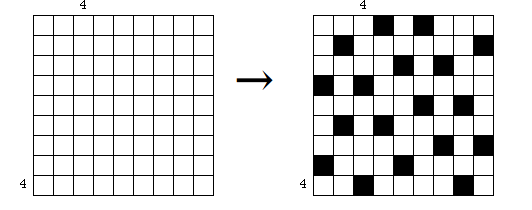
\includegraphics[width=\textwidth]{images/figure1.png}
\caption{Gap Puzzle example} \label{fig1}
\end{figure}
    
\paragraph{}
Although they are very interesting, these specific puzzles do not interest us. We are interested in finding arbitrary 
solutions for a problem with a given order.


\section{Approach}

\subsection{Decision Variables}

\subsection{Constraints}

\section{Search Strategy}


\section{Solution Presentation}
\paragraph{}
For solution presentation there the \textbf{display\_gap(+Sol,+Len)} was elaborated. This predicate receives the \textit{Sol}
list, which is a prolog list containing the coordinates of all grid cells to be shaded for that solution, and \textit{Len},
which is the length of a row, that is, the order of the board the solution given applies to. In order to do this, this 
predicate uses the three predicates explained bellow.

\paragraph{}
This predicate uses the \textbf{empty\_board(-B,+Len)} which creates a list of lists representing an empty grid, with order \textit{Len},
this new grid is then unified with \textit{B}. This predicate works by appending new atoms, representing an empty cell (\textbf{' '}, 
a single space character) to an empty starting list. Once this list has the desired length, this list is then replicated 
several times to form a new empty grid.

\paragraph{}
Then, we use the \textbf{process\_board(+Board,+Sol,-NewBoard)} to substitute all the empty cells in the positions given
by solution list, with the \textbf{'X'} atom. This represents a shaded cell. In order to make the substitution we defined
the \textbf{replaceN(+List,+N,+NewElem,Res)} predicate. This predicate substitutes the element of order \textit{N} in 
\textit{List} to the element \textit{NewElem}, then unifies the resulting list with \textit{NewBoard}.

\paragraph{}
Finally, the predicate \textbf{display\_board(+Board)} was defined to display the board \textit{Board}. This predicate
writes the separators in the screen and then displays each row of the grid, using the right format. Bellow, we can see a
displayed board.
    
\begin{figure}
    \begin{center}
        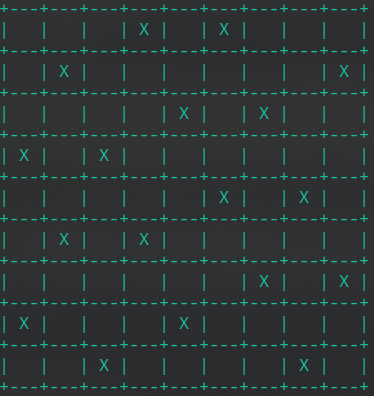
\includegraphics[scale=0.5]{images/fig2.png}
        \caption{Solution Display Example} \label{fig2}
    \end{center}
\end{figure}
    

\section{Results}


\section{Conclusions and Future Work}


\begin{thebibliography}{8}
    \bibitem{ref_url}
    Erich Friedman's Puzzle Palace - Gap Puzzles, Copyright Erich Friedman, 2010. 
    \url{https://www2.stetson.edu/~efriedma/puzzle/gap/}. 
    Last accessed 4 Jan 2020
    \end{thebibliography}

























% Article sampkes  REMOVE IN THE END
\section{Introduction}
\subsection{A Subsection Sample}
Please note that the first paragraph of a section or subsection is
not indented. The first paragraph that follows a table, figure,
equation etc. does not need an indent, either.

Subsequent paragraphs, however, are indented.

\subsubsection{Sample Heading (Third Level)} Only two levels of
headings should be numbered. Lower level headings remain unnumbered;
they are formatted as run-in headings.

\paragraph{Sample Heading (Fourth Level)}
The contribution should contain no more than four levels of
headings. Table~\ref{tab1} gives a summary of all heading levels.

\begin{table}
\caption{Table captions should be placed above the
tables.}\label{tab1}
\begin{tabular}{|l|l|l|}
\hline
Heading level &  Example & Font size and style\\
\hline
Title (centered) &  {\Large\bfseries Lecture Notes} & 14 point, bold\\
1st-level heading &  {\large\bfseries 1 Introduction} & 12 point, bold\\
2nd-level heading & {\bfseries 2.1 Printing Area} & 10 point, bold\\
3rd-level heading & {\bfseries Run-in Heading in Bold.} Text follows & 10 point, bold\\
4th-level heading & {\itshape Lowest Level Heading.} Text follows & 10 point, italic\\
\hline
\end{tabular}
\end{table}


\noindent Displayed equations are centered and set on a separate
line.
\begin{equation}
x + y = z
\end{equation}
Please try to avoid rasterized images for line-art diagrams and
schemas. Whenever possible, use vector graphics instead (see
Fig.~\ref{fig1}).

\begin{figure}
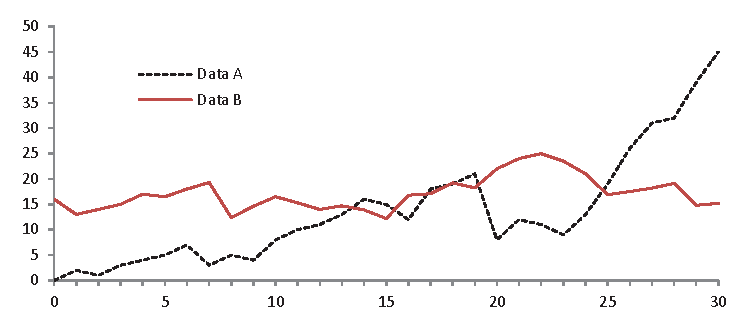
\includegraphics[width=\textwidth]{fig1.eps}
\caption{A figure caption is always placed below the illustration.
Please note that short captions are centered, while long ones are
justified by the macro package automatically.} \label{fig1}
\end{figure}

\begin{theorem}
This is a sample theorem. The run-in heading is set in bold, while
the following text appears in italics. Definitions, lemmas,
propositions, and corollaries are styled the same way.
\end{theorem}
%
% the environments 'definition', 'lemma', 'proposition', 'corollary',
% 'remark', and 'example' are defined in the LLNCS documentclass as well.
%
\begin{proof}
Proofs, examples, and remarks have the initial word in italics,
while the following text appears in normal font.
\end{proof}
For citations of references, we prefer the use of square brackets
and consecutive numbers. Citations using labels or the author/year
convention are also acceptable. The following bibliography provides
a sample reference list with entries for journal
articles~\cite{ref_article1}, an LNCS chapter~\cite{ref_lncs1}, a
book~\cite{ref_book1}, proceedings without editors~\cite{ref_proc1},
and a homepage~\cite{ref_url1}. Multiple citations are grouped
\cite{ref_article1,ref_lncs1,ref_book1},
\cite{ref_article1,ref_book1,ref_proc1,ref_url1}.
%
% ---- Bibliography ----
%
% BibTeX users should specify bibliography style 'splncs04'.
% References will then be sorted and formatted in the correct style.
%
% \bibliographystyle{splncs04}
% \bibliography{mybibliography}
%
\begin{thebibliography}{8}
\bibitem{ref_article1}
Author, F.: Article title. Journal \textbf{2}(5), 99--110 (2016)

\bibitem{ref_lncs1}
Author, F., Author, S.: Title of a proceedings paper. In: Editor,
F., Editor, S. (eds.) CONFERENCE 2016, LNCS, vol. 9999, pp. 1--13.
Springer, Heidelberg (2016). \doi{10.10007/1234567890}

\bibitem{ref_book1}
Author, F., Author, S., Author, T.: Book title. 2nd edn. Publisher,
Location (1999)

\bibitem{ref_proc1}
Author, A.-B.: Contribution title. In: 9th International Proceedings
on Proceedings, pp. 1--2. Publisher, Location (2010)

\bibitem{ref_url1}
LNCS Homepage, \url{http://www.springer.com/lncs}. Last accessed 4
Oct 2017
\end{thebibliography}
\end{document}
